\chapter{\quad Aplicaciones}
En este capítulo se darán los conceptos básicos de teoría de códigos. Se empezará dando una descripción del sistema de comunicación como lo propuso Claude E. Shannon \footnote{Claude Elwood Shannon (Míchigan, 30 de abril de 1916 - 24 de febrero de 2001) fue un ingeniero electrónico y matemático estadounidense, recordado como «el padre de la teoría de la información»} en 1948. En esta parte también se introducirán todos los conceptos básicos del sistema de comunicación como canal, codificador, decodificador y código. Una vez la teoría básica está dada se hace un breve estudio de los códigos lineales, para terminar este capítulo con una clase de códigos en particular, los cíclicos. 

\section{\quad Sistema de Comunicación}
La figura \ref{fig:sistemaComunicacion} muestra un sistema de comunicación de una \textbf{fuente} a un \textbf{destino} mediante un \textbf{canal}. La comunicación puede ser en el dominio del espacio - es decir, de un punto a otro - o en el dominio del tiempo - es decir, al guardar información en algún punto en el tiempo para ser recuperada posteriormente-.
\begin{figure}
\centering
\caption{Sistema de Comunicación propuesto por Shannon}
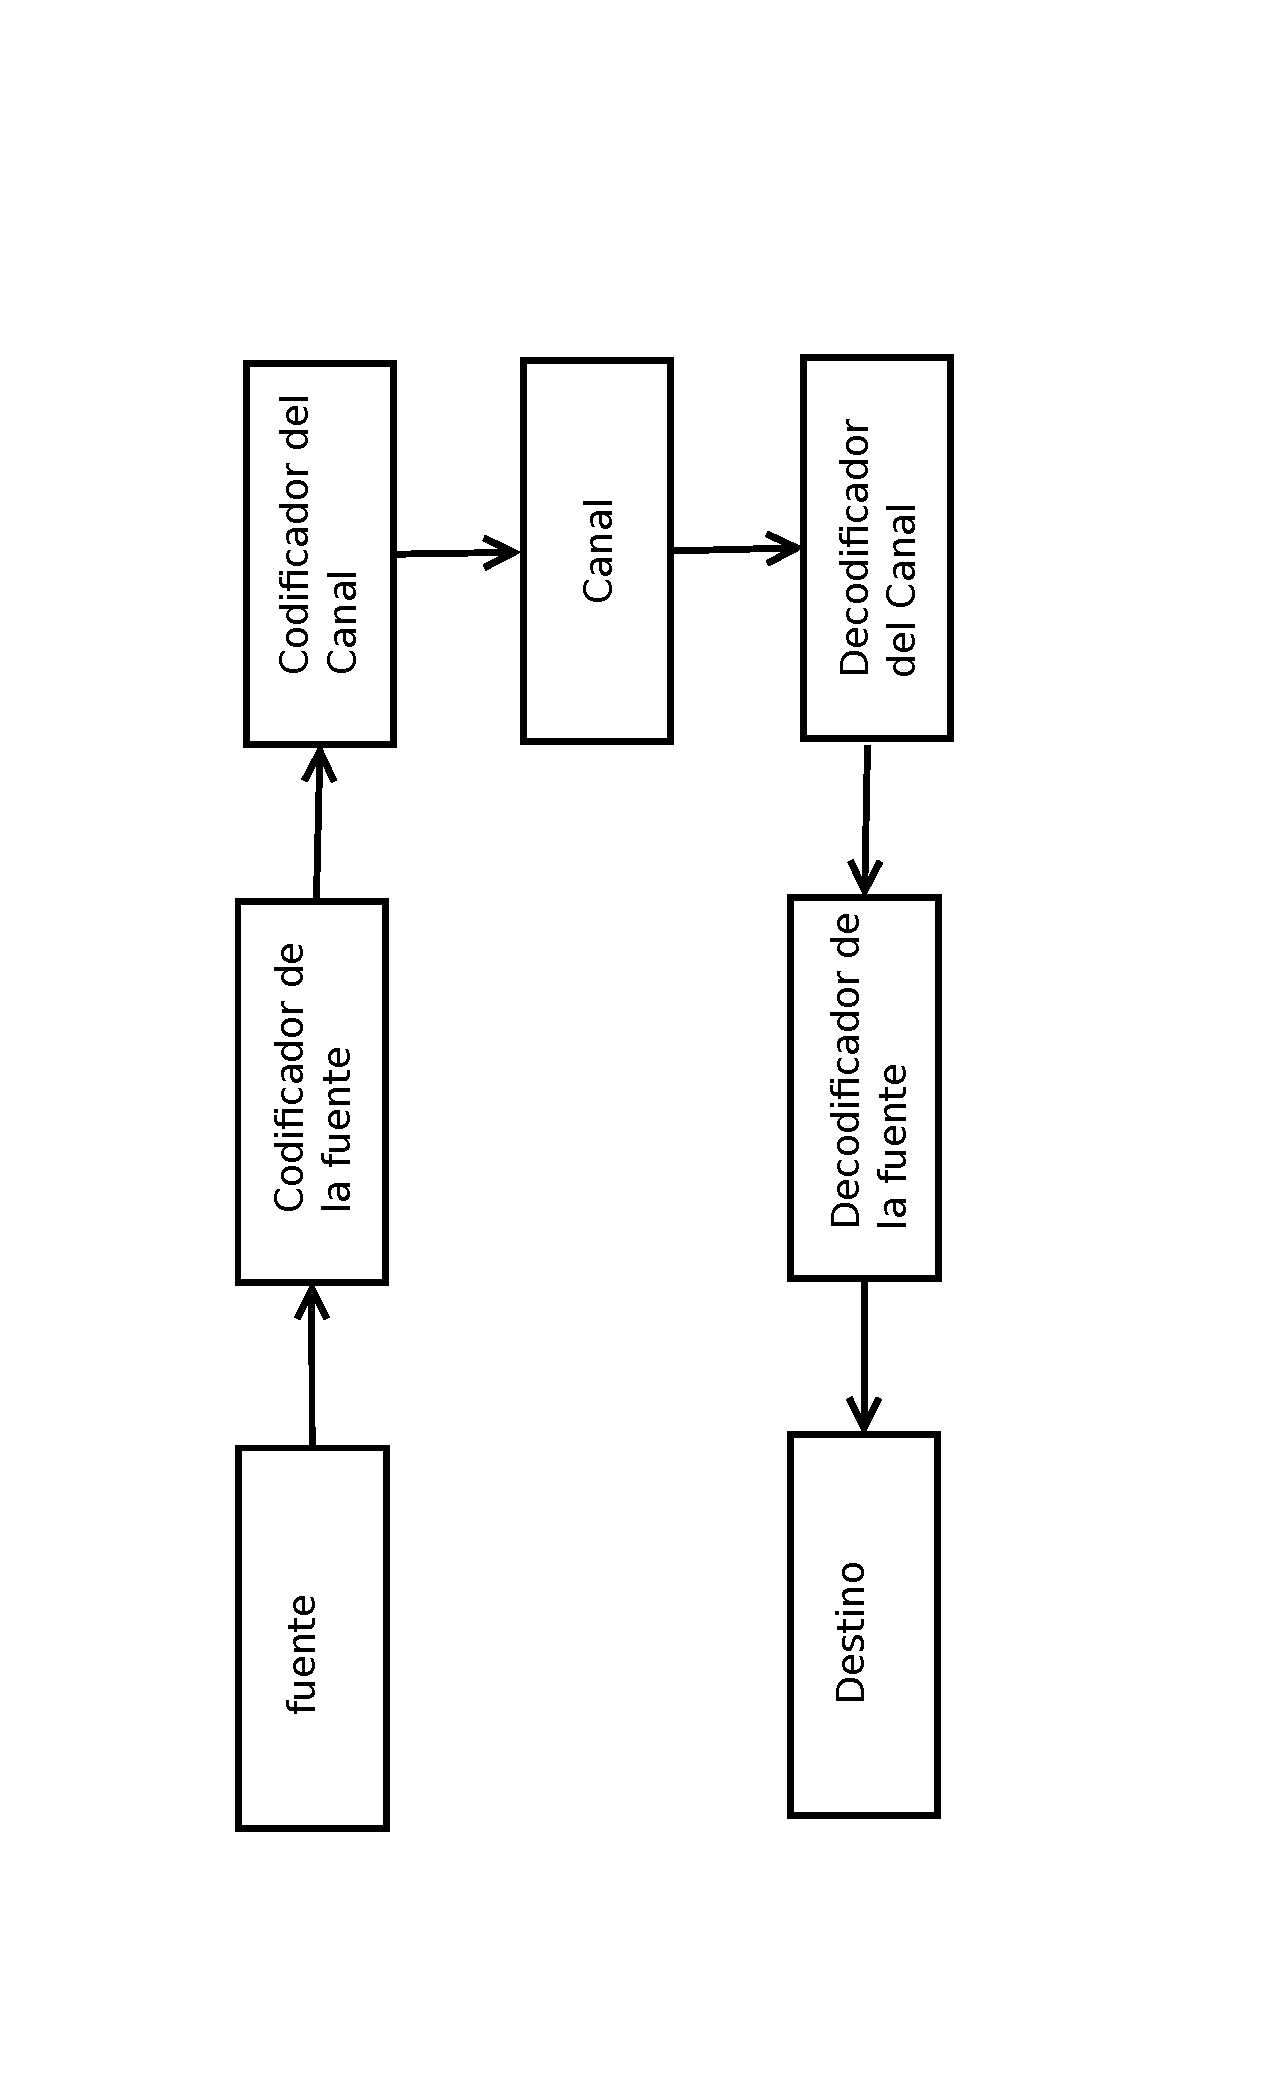
\includegraphics[angle=-90,width=0.7\linewidth]{sistema.pdf}
\caption*{Fuente: Elaboración propia con software Dia.}
\label{fig:sistemaComunicacion}
\end{figure}
La codificación de la fuente tiene doble propósito. Primero, servir como traductor entre la salida de la fuente y la entrada al canal. Por ejemplo, si la información transmitida de la fuente al destino está en señal análoga y el canal espera recibir señal digital, se necesitará una conversión de análoga a digital en la fase de codificación y un convertidor de señal digital a análoga en la fase de decodificación. Como segunda función se podría requerir que el codificador de la fuente comprima la salida de la fuente para economizar en la longitud de la transmisión, eso significa que en el otro extremo, el decodificador de la fuente necesitará descomprimir la señal.

Algunas aplicaciones necesitan que el decodificador restaure la información para que sea idéntica a la original, en cuyo caso se dice que la compresión es \textbf{sin pérdidas}.

Otras aplicaciones, como la mayoría de transmisiones de audio e imágenes, permiten una diferencia -controlada- o distorsión entre la información original y la restaurada, así que esta posibilidad es usada para lograr mayor compresión. En este caso se dice que la compresión es \textbf{con pérdidas.}

Los canales no son perfectos debido a limitaciones físicas y de ingeniería, es decir, su salida puede diferir de su entrada debido al ruido o a defectos de fabricación.

Más aún, en algunos casos el diseño requiere que el formato de la información de salida del canal difiera del formato de entrada. Además hay aplicaciones tales como los medios de almacenamiento masivo magnético y óptico, donde no se permiten ciertos patrones en el flujo de bits a transmitir. Dado esto, el rol principal del codificador del canal, es superar estas limitaciones y hacer el canal tan transparente  como sea posible, tanto desde el punto de vista de la fuente como del destino. 

Es así como entran a participar los códigos. Los códigos fueron inventados para corregir errores en los canales de comunicación debido al ruido. Por ejemplo, supóngase que hay un cable telegráfico desde Ciudad de Guatemala hasta Ciudad de Panamá, mediante el cual se pueden transmitir unos y ceros. Usualmente cuando un cero es enviado se recibe un cero, pero ocasionalmente un cero puede ser recibido como un uno o un uno como un cero. Supóngase que en promedio, 1 de cada 100 símbolos se recibe de forma errónea, es decir, por cada símbolo hay una probabilidad $p=1/100$ de que ocurra un error en el canal. A esto se le llama un canal binario simétrico y se denota como BSC.
\begin{figure}
\centering
\caption{Canal Binario Simétrico}
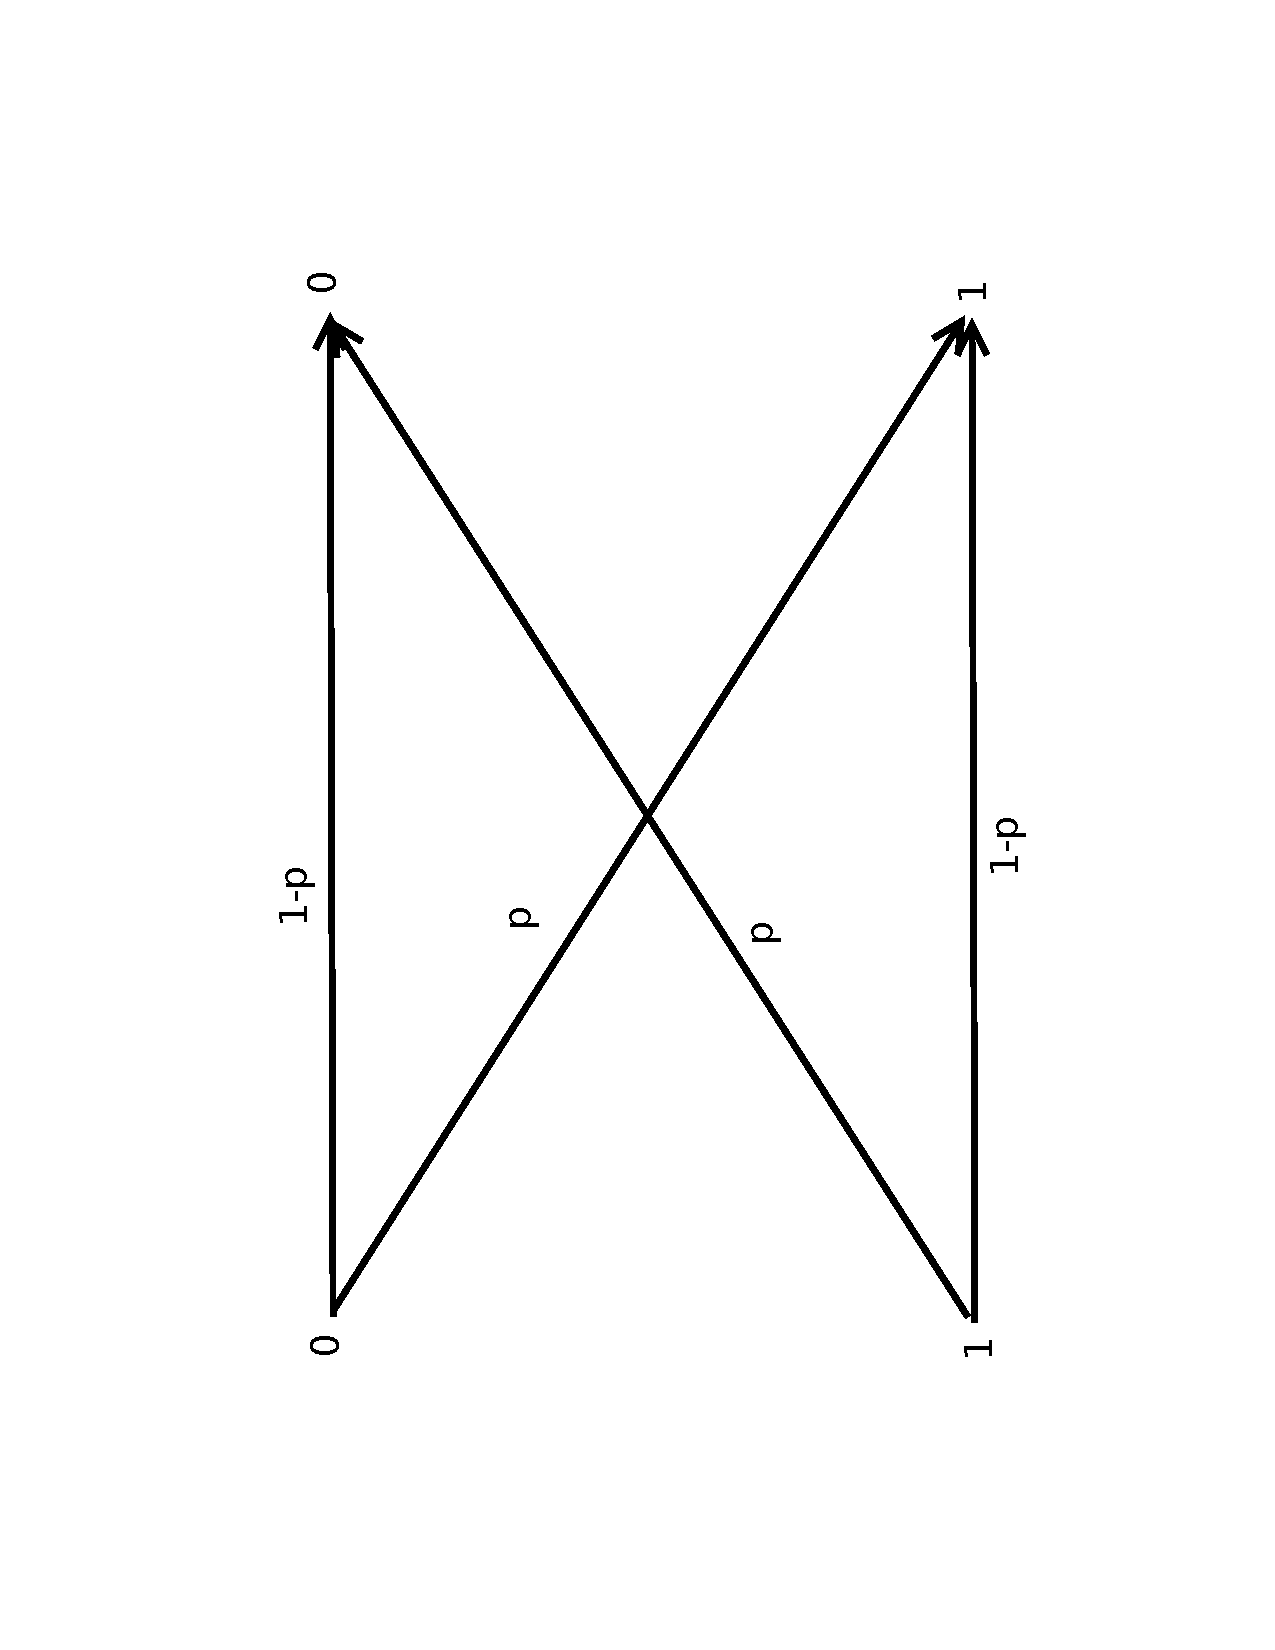
\includegraphics[angle=-90,width=0.6\linewidth]{CBS.pdf}
\caption*{Fuente: Elaboración propia con software Dia.}
\label{fig:CBS}
\end{figure} 
Además supóngase que se enviarán muchos mensajes importantes por ese cable y se necesita enviarlos de manera rápida y segura. Los mensajes ya se encuentran escritos como cadenas de ceros y unos, producidos, quizás, por alguna computadora.

Se van a \textbf{codificar} estos mensajes para darles una protección en contra del ruido del canal. Un bloque de $k$ símbolos del mensaje $u = u_1\dots u_k,\ u_i = 0 \mbox{ o } 1$, será codificado como una \textbf{palabra-código} $x = x_1 \dots x_n, x_i = 0 \mbox{ o } 1$ donde $n \geq k$ (véase la figura \ref{fig:codificacion}). Estas palabra-códigos forman un código.
\begin{figure}
\caption{Proceso de Codificación}
\centering
% Graphic for TeX using PGF
% Title: /mnt/DataWin/Dropbox/Tesis/Tesis Actual/codi.dia
% Creator: Dia v0.97.2
% CreationDate: Wed Dec 11 21:23:59 2013
% For: hugo
% \usepackage{tikz}
% The following commands are not supported in PSTricks at present
% We define them conditionally, so when they are implemented,
% this pgf file will use them.
\ifx\du\undefined
  \newlength{\du}
\fi
\setlength{\du}{15\unitlength}
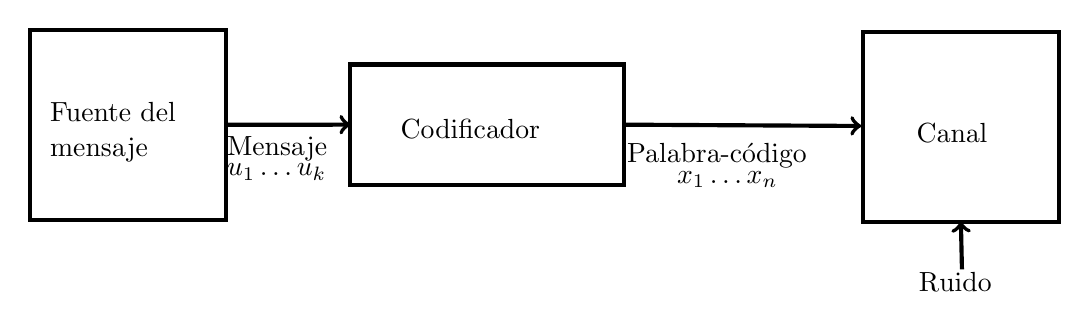
\begin{tikzpicture}
\pgftransformxscale{0.800000}
\pgftransformyscale{-0.700000}
\definecolor{dialinecolor}{rgb}{0.000000, 0.000000, 0.000000}
\pgfsetstrokecolor{dialinecolor}
\definecolor{dialinecolor}{rgb}{1.000000, 1.000000, 1.000000}
\pgfsetfillcolor{dialinecolor}
\pgfsetlinewidth{0.100000\du}
\pgfsetdash{}{0pt}
\pgfsetdash{}{0pt}
\pgfsetmiterjoin
\definecolor{dialinecolor}{rgb}{1.000000, 1.000000, 1.000000}
\pgfsetfillcolor{dialinecolor}

\definecolor{dialinecolor}{rgb}{0.000000, 0.000000, 0.000000}
\pgfsetstrokecolor{dialinecolor}
\draw (3.731981\du,6.945629\du)--(3.731981\du,13.482575\du)--(9.631981\du,13.482575\du)--(9.631981\du,6.945629\du)--cycle;
% setfont left to latex
\definecolor{dialinecolor}{rgb}{0.000000, 0.000000, 0.000000}
\pgfsetstrokecolor{dialinecolor}
\node[anchor=west] at (4.006981\du,9.767031\du){Fuente del };
% setfont left to latex
\definecolor{dialinecolor}{rgb}{0.000000, 0.000000, 0.000000}
\pgfsetstrokecolor{dialinecolor}
\node[anchor=west] at (4.006981\du,11.089242\du){mensaje};
\pgfsetlinewidth{0.100000\du}
\pgfsetdash{}{0pt}
\pgfsetdash{}{0pt}
\pgfsetmiterjoin
\definecolor{dialinecolor}{rgb}{1.000000, 1.000000, 1.000000}
\pgfsetfillcolor{dialinecolor}
\definecolor{dialinecolor}{rgb}{0.000000, 0.000000, 0.000000}
\pgfsetstrokecolor{dialinecolor}
\draw (13.386981\du,8.142031\du)--(13.386981\du,12.282031\du)--(21.636981\du,12.282031\du)--(21.636981\du,8.142031\du)--cycle;
% setfont left to latex
\definecolor{dialinecolor}{rgb}{0.000000, 0.000000, 0.000000}
\pgfsetstrokecolor{dialinecolor}
\node[anchor=west] at (14.561981\du,10.357031\du){Codificador};
\pgfsetlinewidth{0.100000\du}
\pgfsetdash{}{0pt}
\pgfsetdash{}{0pt}
\pgfsetbuttcap
{
\definecolor{dialinecolor}{rgb}{0.000000, 0.000000, 0.000000}
\pgfsetfillcolor{dialinecolor}
% was here!!!
\pgfsetarrowsstart{to}
\definecolor{dialinecolor}{rgb}{0.000000, 0.000000, 0.000000}
\pgfsetstrokecolor{dialinecolor}
\draw (13.386981\du,10.212031\du)--(9.631981\du,10.214102\du);
}
\pgfsetlinewidth{0.100000\du}
\pgfsetdash{}{0pt}
\pgfsetdash{}{0pt}
\pgfsetbuttcap
{
\definecolor{dialinecolor}{rgb}{0.000000, 0.000000, 0.000000}
\pgfsetfillcolor{dialinecolor}
% was here!!!
\pgfsetarrowsstart{to}
\definecolor{dialinecolor}{rgb}{0.000000, 0.000000, 0.000000}
\pgfsetstrokecolor{dialinecolor}
%line i am interested in
\draw (28.770935\du,10.256598\du)--(21.636981\du,10.212031\du);
}
% setfont left to latex
\definecolor{dialinecolor}{rgb}{0.000000, 0.000000, 0.000000}
\pgfsetstrokecolor{dialinecolor}
\node[anchor=west] at (9.331981\du,11.042031\du){Mensaje};
% setfont left to latex
\definecolor{dialinecolor}{rgb}{0.000000, 0.000000, 0.000000}
\pgfsetstrokecolor{dialinecolor}
\node[anchor=west] at (9.331981\du,11.842031\du){$u_1\dots u_k$};
% setfont left to latex
\definecolor{dialinecolor}{rgb}{0.000000, 0.000000, 0.000000}
\pgfsetstrokecolor{dialinecolor}
\node[anchor=west] at (21.381981\du,11.292031\du){Palabra-código};
% setfont left to latex
\definecolor{dialinecolor}{rgb}{0.000000, 0.000000, 0.000000}
\pgfsetstrokecolor{dialinecolor}
\node[anchor=west] at (22.881981\du,12.092031\du){$x_1\dots x_n$};
\pgfsetlinewidth{0.100000\du}
\pgfsetdash{}{0pt}
\pgfsetdash{}{0pt}
\pgfsetmiterjoin
\definecolor{dialinecolor}{rgb}{1.000000, 1.000000, 1.000000}
\pgfsetfillcolor{dialinecolor}
\definecolor{dialinecolor}{rgb}{0.000000, 0.000000, 0.000000}
\pgfsetstrokecolor{dialinecolor}
\draw (28.820292\du,7.014162\du)--(28.820292\du,13.551108\du)--(34.720292\du,13.551108\du)--(34.720292\du,7.014162\du)--cycle;
% setfont left to latex
\definecolor{dialinecolor}{rgb}{0.000000, 0.000000, 0.000000}
\pgfsetstrokecolor{dialinecolor}
\node[anchor=west] at (30.099923\du,10.484211\du){Canal};
% setfont left to latex
\definecolor{dialinecolor}{rgb}{0.000000, 0.000000, 0.000000}
\pgfsetstrokecolor{dialinecolor}
\node[anchor=west] at (30.168743\du,15.632869\du){Ruido};
\pgfsetlinewidth{0.100000\du}
\pgfsetdash{}{0pt}
\pgfsetdash{}{0pt}
\pgfsetbuttcap
{
\definecolor{dialinecolor}{rgb}{0.000000, 0.000000, 0.000000}
\pgfsetfillcolor{dialinecolor}
% was here!!!
\pgfsetarrowsstart{to}
\definecolor{dialinecolor}{rgb}{0.000000, 0.000000, 0.000000}
\pgfsetstrokecolor{dialinecolor}
\draw (31.770292\du,13.551108\du)--(31.802718\du,15.192715\du);
}
\end{tikzpicture}

\caption*{Fuente: Elaboración propia con software Dia y exportado a \TeX}
\label{fig:codificacion}
\end{figure}
La primera parte de la palabra-código consiste en ele mensaje mismo: \[ x_1 = u_1,\ x_2 = u_2,\ \dots ,\ x_k = u_k, \] seguido de $n-k$ símbolos de comparación $x_{k+1}, \dots , x_n$. 
Los símbolos de comparación son elegidos de tal forma que las palabra-códigos satisfagan 
\[ H \begin{pmatrix}
x_1 \\ 
x_2 \\
\vdots \\
x_n
\end{pmatrix} = Hx^{t} = 0, \] donde la matriz $H$ de $(n-k)\times k$ es la matriz de comparación de paridad del código, dada por 
\begin{equation}\label{ecu:defCodigo}
H = [A \mid I_{n-k}],
\end{equation}  
donde $A$ es una matriz fija de $(n-k)\times k$ de ceros y unos y \[ I = \begin{pmatrix}
1 & 0 & \dots & 0 \\
0 & 1 & \dots & 0 \\
\vdots & \vdots & \ddots & \vdots \\
0 & 0 & \dots & 1
\end{pmatrix} \] es la matriz identidad de $(n-k) \times (n-k)$. La aritmética en la ecuación \ref{ecu:defCodigo} se hace en módulo 2, es decir que se está trabajando con el campo $\mathds{Z}_2$. 
\begin{ejemplo}
La matriz de comparación de paridad 
\[ H = \left(\begin{array}{ccc|ccc}
0 & 1 & 1 & 1 & 0 & 0 \\
1 & 0 & 1 & 0 & 1 & 0 \\
1 & 1 & 0 & 0 & 0 & 1
\end{array}\right) \] define un código con $k=3$ y $n=6$. Para este código 
\[ A = \begin{pmatrix}
0 & 1 & 1\\
1 & 0 & 1 \\
1 & 1 & 0
\end{pmatrix}.  \]
El mensaje $u_1u_2u_3$ es codificado en la palabra-código $x = x_1x_2x_3x_4x_5x_6$ que empieza con el propio mensaje:
\[ x_1 = u_1, x_2 = u_2, x_3 = u_3, \] seguido de tres símbolos de comparación $x_4x_5x_6$ tales que $Hx^t = 0$, es decir, se cumple
\begin{eqnarray}\label{ecu:comparacion}
x_2 + x_3 + x_4 = 0, \\
x_1 + x_3 + x_5 = 0, \\
x_1 + x_2 + x_6 = 0.
\end{eqnarray}
Si el mensaje es $u = 011$, entonces $x_1= 0,\  x_2 = 1, \ x_3 =1$ y los símbolos de comparación son
\begin{eqnarray*}
x_4 & = & 0 \\
x_5 &=& 1 \\
x_6 &=& 1
\end{eqnarray*}
por lo que la palabra-código es $x = 011011$.
\end{ejemplo}
Las ecuaciones \ref{ecu:comparacion} son llamadas ecuaciones de comparación de paridad del código. Las ecuaciones de paridad dicen que el cuarto, quinto y sexto símbolo siempre deben sumar cero módulo 2, es decir, su suma siempre es par. 

Es fácil notar que el número de palabra-códigos posibles para esta matriz es $2^3 = 8$. Estas son:
\[ \begin{array}{ccc}
000000 & 011011 & 110110 \\
001110 & 100011 & 111000 \\
010101 & 101101 & 
\end{array}. \]
En general en un código hay $2^k$ palabra-códigos, si el alfabeto es $\{0,1\}$.

Luego de haber visto de manera intuitiva un código lineal, se da la definición formal:
\begin{definicion}
Un código de bloques lineal sobre GF(q) de longitud $n$ y dimensión $k$, es un subespacio de de $V_n(q)$ de dimensión $k$, donde $V_n(q)$ es un espacio vectorial de dimensión $n$ sobre GF(q). Se denota a este como código lineal $(n,k)$.
\end{definicion}
El término código de bloques se refiere al hecho que toda palabra-código tiene la misma longitud, es decir, es una $n\mbox{-upla}$. La palabra lineal se deriva del simple hecho que las palabra-códigos forman un subespacio. 
También existen los códigos de árbol, de los cuales los códigos de convolución son un caso especial. Dichos códigos no dividen el mensaje en bloques. En la práctica de la ingeniería estos códigos son bastante importantes, pero no se hablará de estos en este trabajo.
\begin{definicion}
La distancia de Hamming $d(u,v)$ entre dos $n\mbox{-uplas}$ $u$ y $v$ de $V_n(q)$ está definida como el número de coordenadas en el cual difieren. El peso de Hamming $\omega(u)$ de una $n\mbox{-upla } u \in V_n(q)$ es el número de coordenadas no nulas de $u$.
\end{definicion}
La mayor parte del trabajo en teoría de códigos se desarrolla en base a la distancia de Hamming. Otra métrica con la que también se trabaja es la de Lee.

Como se dijo anteriormente, en la transmisión de una palabra-código en algún canal se puede producir errores debido al ruido. Por error, se entiende que puede ocurrir un cambio en cualquiera de las coordenadas de la $n\mbox{-upla}$ trasmitida. Justamente el punto de codificar es que, bajo ciertas circunstancias, estos errores se pueden corregir.

\section{\quad Códigos Cíclicos} 

Ya que se ha hecho la presentación de los códigos lineales, se procede a estudiar una clase muy particular e importante de ellos; los códigos cíclicos.

\begin{definicion}
Un código es cíclico si es lineal y además todo desplazamiento cíclico de las coordenadas de una palabra-código es también una palabra-código. 
\end{definicion}
Los códigos cíclicos figuran entre los primeros que aparecieron para el uso práctico, estos eran implementados usando registros de desplazamientos\footnote{Un registro de desplazamiento es un circuito digital secuencial - es decir, que los valores de sus salidas dependen de sus entradas y de los valores anteriores-  consistente en una serie de biestables, generalmente de tipo D, conectados en cascada , que basculan de forma sincrónica con la misma señal de reloj. Según las conexiones entre los biestables, se tiene un desplazamiento a la izquierda o a la derecha de la información almacenada. Es de señalar que un desplazamiento a la izquierda de un conjunto de bits, multiplica por 2, mientras que uno a la derecha, divide entre 2. Existen registros de desplazamiento bidireccionales, que pueden funcionar en ambos sentidos. Los registros universales, además de bidireccionales permiten la carga en paralelo.}. 
Para poder hacer un buen diseño de códigos es necesario conocer la estructura algebraica de los mismos. en esta sección se abordará la estructura algebraica de los códigos cíclicos.
El lector deberá notar que los códigos cíclicos no dependen de la linealidad de los mismos, de hecho, también existen los códigos cíclicos no lineales.

Resulta muy conveniente identificar a los códigos cíclicos con polinomios, esto es, a cada palabra-código
\[ a = (a_0, a_1, \dots , a_{n-1}) \in \mathds{F}^n \] se le asocia el polinomio \[ a(x) = a_0 + a_1x+ \cdots + a_{n-1}x^{n-1} \in \mathds{F}[x]_n .\] Si $c$ es una palabra-código del código $\mathcal{C}$, entonces $c(x)$ es sus polinomio-código asociado. Con esta identificación, la palabra-código con corrimiento $\tilde{c}$ tiene el polinomio-código asociado \[ \tilde{c}(x) = c_{n-1} + c_0x + c_1x^2 + \cdots + c_{n-2}x^{n-2}. \] Así, es tentador pensar que $\tilde{c}(x) $ es casi igual al producto $xc(x)$. Más aún, 
\[ \tilde{c}(x) = xc(x) - c_{n-1}(x^n -1)  \] de donde se deduce que \[ \tilde{c}(x) = xc(x) (\mbox{mód } x^n-1) .\] Dicho de otra manera $\tilde{c}(x)$y $xc(x)$ son iguales en el anillo de polinomios $\mathds{F}[x]$ con multiplicación módulo $x^n-1$. Como se esta trabajando con códigos, según la definición $\mathds{F} = GF(q) $ y $GF(q)[x]$ es el anillo de polinomios sobre $GF(q)$ en la variable $x$. Entonces, por lo dicho en el párrafo anterior, resulta claro que hay un isomorfismo natural entre $GF(q)[x]/(x^n-1)$ y los polinomios de grado menor que $n$ con multiplicación definida módulo $x^n-1$. Se denota al anillo $GF(q)[x]/(x^n-1)$ como $A_n$. Es claro que $A_n$ es también un álgebra sobre $GF(q)$. Más aún, si $C_n = \langle x \rangle,\ x^n =1$, es un grupo cíclico de orden $n$, es evidente que existe un isomorfismo entre $GF(q)C_n$ y $GF(q)[x]/(x^n-1) = A_n$, donde se ha utilizado el símbolo $x$ para ambas álgebras con el único propósito de hacer énfasis en esta identificación.
Lo anterior quiere decir que $A_n \simeq GF(q)C_n$, pero $GF(q)C_n$ es un grupo-álgebra, con lo cula se ha demostrado que los códigos cíclicos son un grupo-álgebra y por lo tanto su estructura algebraica está plenamente identificada. Además se tiene el siguiente teorema:
\begin{teorema}
Un código $(n,k) \ \mathcal{C}$ sobre $GF(q)$ es lineal si y sólo si dicho código es un ideal de $A_n$.
\end{teorema}
\begin{proof}
Sea $\mathcal{C}$ un ideal de $A_n$. Es claro que $\mathcal{C}$ es un subespacio de $A_n$ como espacio vectorial, por lo que solamente falta verificar que es un subespacio cíclico, lo cual se sigue del hecho que $\mathcal{C}$ es ideal y por lo tanto cerrado bajo multiplicación por $x$.
Para el converso, supóngase que $\mathcal{C}$ es un subespacio cíclico, eso quiere decir que es cerrado bajo la suma y el producto por $x$ y por lo tanto es cerrado bajo el producto de cualquier elemento de $A_n$, entonces $\mathcal{C}$ es un ideal.
\end{proof}
Como el lector podrá notar, el estudio de códigos lineales, se reduce a estudiar los ideales de $A_n$, que es un grupo-álgebra. Para ello será provechoso conocer cuando $A_n$ es semisimple o no, tarea que se realizó en el capítulo 3. 



